\section{Target Description}



Northern Gujarat is a marginal environment between the Thar Desert and the more fertile area of
Saurashtra. This region is an ecotone, characterized by the seasonal influence of the monsoon where
contrasting ecological niches are in tension and small climatic shifts can generate significant
environmental changes, eventually affecting resource availability. Archaeological evidence points to
the presence and possible coexistence in the area of groups of people with different resource
management strategies and mobility behaviors: hunter-gatherers (HG); agropastoralists (AP).
The aim of this study is to model resource management and decision making among hunter-gatherer
groups in this region to explore adaptive trajectories and performance in relation to a) environmental
variability and b) the appearance of other specialized groups.
What factors play a role in HG persistence or disappearance in arid margins? Is the advent of agro-
pastoral behaviour a big enough change to explain the disappearance of HG behaviour? Does climate
variability affect HG behaviour?
The model description follows the ODD (Overview, Design concepts, Details) protocol for describing
individual- and agent-based models (Grimm et al. 2006, 2010).

Note:
The modeling workflow is following these steps:
1. Environmental settings and climate engine
2. Resources and energy flow
3. Socio-ecological behaviour of HG
4. Socio-ecological behaviour of AP
5. Cultural transmission

This scaling approach includes three main theoretical and methodological research aspects:
1. Human behavioral ecological approach and socio-ecological co-evolutionary framework
2. Model based vs rule based action planner of the agents
Up to the date, steps 1, 2 and 3 have been developed . Work regarding AP models and cultural
transmission is in progress.


\section{Purpose}
In our starting hypothesis HG groups are adapted to marked seasonality (represented by the
monsoon) in the arid margins of northern Gujarat. We intend to explore HG resilience (Holling 1973,
Carpenter et al. 2001) considering: a) the appearance of AP, b) climate variability.

\section{Entities, state variables, scales}
The model initially explores separately socio-ecological behaviours of two isolated populations: 1)
Hunter-Gatherers (HG) agents and 2) Agro-Pastoralist (AP) agents. This separate simulation of the
two groups is needed to obtain independent, coherent and consistent models of HG and AP decision
making. Once the dynamics of the modeled systems are understood for each population, agents from
the two populations will be combined in a single simulation execution. These will be considered as
independent groups, and interaction between agents will be limited to other agents belonging to the
same population.
Agents from one population will interact within a given territory. It is characterised in terms of: a)
geographical information derived (height, slope), and b) landscape (soil types, resources). This
territory and its characteristics will generate an environment that will allow to portray differences in
strategies regarding settlement, mobility and resource use.

\subsection{Scales}
\paragraph{Agent Scale}

For both populations (AP and HG) the basic agent is defined as a couple (one woman and one man).
This is considered to be the entity engaging in all decision-making processes and actions that will be
modelled in the simulation.

\paragraph{Time Scale}
Time Scale for the simulation is one day. This time step is coherent with the granularity of agents’
planning.
\paragraph{Space Scale}
The spatial resolution of the proposed simulation model is constrained by the resolution of available
relevant geographic data and the nature of the agent mobility and resource gathering activities being
modelled.
Hence, it was decided to use 31.5m x 31.5m cells, corresponding to ca. 1,000 square meters. First
and most important, this is the level of resolution of the most detailed geographical information
available for the area; second, this surface can fit the type of settlements recognised from the
archaeological surveys.

\subsection{Environment}
The simulation environment is large enough to develop all potential processes defined by the model. It
extends over an area of 25 Km x 25 Km (625 Km2). Space is represented as a regularly spaced grid
of cells (a raster map). Each cell is a square of 31.5 m per side, and the total size of this environment
translates into a space of 800 x 800 cells (25,200 m x 25,200 m).
The ground model includes elevation and land features. Elevation is determined by a Digital Elevation
Model (DEM), a raster map containing the elevation value for each cell calculated from contemporary
satellite imagery. Land characteristics are reduced to three elemental features:

\begin{enumerate}
\item Water Body: represents rivers and lakes.
\item Sand Dune: represents the top area of the dune, which can be settled. Home location of the
agent will always be in a dune cell.
\item Interdunal Soil: represents the interdune area where resources grow. The different land
features do not seasonally change in extension but their productivity (in terms of moist content
and therefore resources supported) does.
\end{enumerate}

The cornerstone of our environmental modeling is the climatic engine. The climate module determines
the quantity of rain that precipitates evenly on the landscape on every time step. Precipitation is used
in conjunction with the terrain model to calculate the amount of biomass for each cell and season. The
climate model is based on present-day, historical and palaeoclimatic data, as well as Holocene
monsoon models.

\subsubsection{Climate}
The focus on the co-evolution of resource utilization strategies within a particular environment requires
to make explicit the potential variations in the landscape. In particular for our case study, the presence
of the monsoon generates a strong seasonality (asymmetrical precipitation patterns).
Monsoon seasonality determines the presence of three critical “moments” in simulation time, each
spanning 4 months. Therefore, the seasonal subdivision in three periods will be repeated in a cyclical
way as follows:

\begin{enumerate}
\item JJAS (rain season: high precipitation, high temperature, low evapotranspiration)
\item ONDJ (post-Monsoon: low precipitation, cool temperature, medium evapotranspiration)
\item FMAM (dry season: low precipitation, high temperature, high evapotranspiration)
\end{enumerate}

It is important to note that any given “year” in the model starts with the beginning of the rain season
(June). In fact, virtually all rain in the region is carried by the monsoon that falls between June and
September (JJAS). Therefore, it is during the JJAS beginning that the totality of the generated yearly
precipitation value will be calculated (following the Weibull distribution). No additional precipitation is
considered for the remaining eight months of the year ( ONDJ and FMAM).


\subsubsection{Resources}
Each cell has a finite number of resources and a type. Any given cell can be:

Wild cell. Resource availability for each cell is calculated from the following variables:

\begin{enumerate}
\item Yearly precipitation (rainfall, the Weibull distribution)
\item Type of cell (Water Body, Interdune, Dune)
\item Mean yearly Biomass per cell and type.
\item Cell history (e.g. whether the cell was used for crop in a previous step or part of the resources
were consumed before).
\end{enumerate}

Wild resources include the total biomass that can be found in a cell (fauna and flora). Wild resources
are exploited by HG agents engaging into foraging activities. Foraging includes activities such as
hunting animals and gathering plants, fruits, seeds, etc. Indeed, from a literature review it is clear that
secondary biomass production (animals) is directly related to primary biomass quantity. Moreover, as
there is no interest in our simulation to explore gender-based labour division we decided to consider
hunting and gathering as a single activity (foraging) without distinguishing between plant or animal
utilization. In the light of this, it was decided to consider a value for wild cell (dune vs interdune) based
on published information of primary biomass production in desert (dune) and savannah (interdune)
biomes (after Kelly 1983 – Table 3).

%%pg4
\begin{table}[ht!]
\centering	
	\begin{tabular}[c]{|l|l|l|l|l|}
	\hline
	CELL TYPE & Yearly Primary Biomass Production & Efficiency & Energy & KCal \\
	\hline
	Dune (desert) & $700g/m^2$ & $13\%$ & $1820KJ/m^2$ & $435KCal$ \\ 
	\hline
	Interdune (savanna) & $4000g/m^2$ & $23\%$ & $18400KJ/m^2$ & $4395KCal$ \\
	\hline
	\end{tabular}
	\caption{Percentage of accessible resources calculated accordingly to Kelly (1983; Table 3, p. 284).}
	\label{tab:tabResources}
\end{table}

\begin{enumerate}
 \item Cell area = 1000m2
 \item 1 g Primary Biomass = 20KJ
 \item 1 kcal = 4.184 KJ
\end{enumerate}


\paragraph{Efficiency}
The total primary biomass value does not constitute the entire primary biomass available for
consumption to animals and humans. This value represents the entire biomass production
including both edible (fruits, tubers some roots etc.) and non-edible (wood, stems, branches
etc.) parts of the plants. The ratio of profitable biomass versus whole biomass will be the
efficiency value specified in the above table that allow to calculate the energy effectively
available for humans.


Domesticated cell (work in progress)
Domesticated plant resources define the density of domesticated plants found inside the cell. It is
important to note that wild and domesticated types of resources are mutually exclusive: i.e. wild
resources are not found on cultivated plots. These cells can have two different states:


resources are not found on cultivated plots. These cells can have two different states:
\begin{enumerate}
\item Crop: The cell is ready for agricultural uses (sow-harvest cycle).
\item Fallow: The cell can't be used for agricultural uses, but is good for grazing.
\end{enumerate}

\begin{figure}[h]
\centering
\setlength\fboxsep{0pt}
\setlength\fboxrule{0.5pt}
\fbox{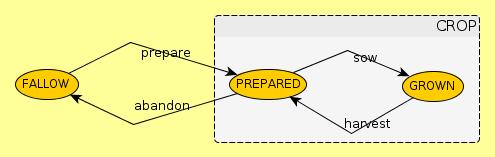
\includegraphics[width=120mm,keepaspectratio=true]{figures/cropStates.jpg}}
\caption{States of a crop and transitions}
\label{fig:cropStates}
\end{figure}


The basic idea for a domestication cell is that of small scale shifting cultivation, in which a plot is
cultivated following a cycle that includes abandonment so to allow soil properties to recover. A
domesticated cell can be planted for a maximum of three consecutive years. It then needs to be
abandoned for a minimum of three years (during which it will be considered as Fallow). After three
years of abandonment the cell becomes wild and can be used again for agriculture. If a plot is
abandoned before being cultivated for three consecutive years it will have to remain abandoned for
the same amount of years it was worked. During these years it will remain fallow, after that it will
become wild again.

Crop cells change temporary their state to Fallow during the FMAM season, where no agricultural
uses can be executed. It turns to Crop again during JJAS season, and will be ready to sow at the end
of it.



\subsection{Agents}
The following attributes have been chosen to account in our model for both HG and AP:

\begin{enumerate}
\item Children – A collection of human entities. The number of children is bound by resource
availability.
\item Home location – The cell were the agent resides. It is the spatial centre of the activities
carried out by the agent. A given cell can be shared by more than one agent from the same
group, be it HG or AP. On the other hand, there is a physical limit (Maximum Homes per
cell) in the number of agents that can settle the same cell (max 20 agents per cell, see HG
Surrogates).
\item Relationships – These are the connections between agents. The following types of
relationship are considered:\\
	\begin{enumerate}
 
	\item Acquaintance – This is the result of having met at some time in the past. A numeric
	value is used to track the intensity of the relationship. This value changes with and
	depends on the actions of the involved agents.\\
	\item Next Of Kin – Agents connected by family ties (the agents have some common
	ancestor). The closeness of the family tie is also modelled with an intensity value that
	remains constant throughout the agent's life. The value is inversely proportional to the
	distance in the genealogical tree.

	\end{enumerate}

\item Surplus – At any point in time, the amount of calories the agent did not use for survival.
\item Age – A numeric variable that keeps track of how many time steps a given agent has been
active in the simulation.
\item Food Needs – A costant that sets the minimum calories a given agent needs in each time
step. This survival threshold can be different for different types of agents.
\end{enumerate}

\subsubsection{Hunter-Gatherer (HG)}
The following attributes are specific for hunter-gatherers:
\begin{enumerate}
\item Home range – The maximum distance an agent will travel in one day. This attribute restricts
foraging activities by not permitting or making it anti-economic to engage in foraging in cells
too far from the agent Home Location. Social activities are also limited in a similar way.
The area enclosed in the circle of radius “Home range” is divided in a predefined number of
sectors. Such division allows to model the idea of direction of exploration for the agent
actions, while simplifying the decision-making process (an agent will choose to forage in one
of the sectors, not particular cells). More details can be found below associated to the
description of actions and the agent decision cycle submodel.

\item Quickness in forage
\item displacement rate...

\end{enumerate}


pg6 grafic home range


\subsubsection{Agro-Pastoralists (AP)} (work in progress)
The following attributes are considered to be specific to agro-pastoralists:

\begin{enumerate}
\item Plot – A cell cultivated by an agent.
\item Herd – The quantity of domesticated animals that the agent owns. Although herds are
resources for Agro-Pastoralists, they have been modelled as an attribute of the agent. The
model keep track of the size of the agent's herd, and it is responsible for grazing the animals
in order to maintain the number and get resources from the herd. This action will use wild and
owned fallow cells inside the Home Range.
\item Maximum plot range – The maximum distance in cells from Home that AP agents are
allowed to go to set up an agricultural plot.
\item Maximum grazing range – The maximum distance in cells from Home that AP agents are
allowed to go for grazing.
\end{enumerate}

AP agents may or may not have both plots and herds.


\section{Process overview and scheduling}
The execution has 2 scales. On the one hand, three processes (‘Yearly Precipitation’, ‘biomass yearly
production’ and ‘Population size adjustment’) are executed once every year. On the other hand,
agents decision-making processes use a daily time step. The simulation follows this schedule,
beginning the first day of a JJAS season:
For each year:

//* indent

1. Precipitation calculation
2. Biomass Yearly Production
3. For each day of the year:
3.a. Daily biomass availability
3.b. Agent planning:
3.b.i. Knowledge update
3.b.ii. Choice of actions
3.c. Execution of agents actions
4. Population size adjustment
Details for each simulation phase are given hereafter.


\subsection{Precipitation calculation}
The total amount of rain is calculated as a random number following the Weibull distribution defined in
section 8 (Input Data)
\subsection{Biomass Yearly Production}
The biomass that a cell will produce in an entire year is calculated from rainfall and mean year
production for its particular type, provided by historical records.
We will consider a lineal relation between rain and biomass production for the sake of simplicity. The
deviation of rain estimated for year from its mean will allow to interpolate the amount of biomass
deviation from the yearly mean biomass. That is, if the mean of rain is 100 liters and the climate model
produces 80 liters the deviation to apply is 20%, and for that year the biomass will be a 80% of the
mean yearly production.

\subsection{Daily processes}

\subsubsection{Biomass availability}
Yearly biomass production will not appear immediately in the cell in the first day of JJAS season.
Resources will gradually increase under the accumulation of water until some days after the end of the
season. It will slowly decrease in the following months, until the beginning of the next rainy season.
Next figure depicts this process as a triangle, being its Height (M) the peak of resources in a given cell,
its Base (L, divided in L1=JJAS and L2=ONDJ+FMAM) the time span of one year, and its area (A) the
yearly biomass production.

pg7 grafic triangle biomass grow

formulae : 
\begin{equation}
	A=B * (H/2)
	A=(L1*M/2)+(L2*M/2)
	A=(L1+L2)*M/2
	M=2A/(L1+L2)
\end{equation}

Finally we calculate the daily ratio of resource grow (JJAS) and decay (ONDJ-FMAM) for each cell as
follows:

	$Grow = M/L1$

	$Decay = -(M/L2)$

\subsubsection{Agent planning}
Each day the agent will update its knowledge about environment and choose a list of actions to
execute (the decision-making process is defined in the Submodels section). The list of available
actions is:


\paragraph{Common to HG \& AP:}

\begin{enumerate}
\item Move Home - The agent moves from its current home location to set up a new one
elsewhere inside Home Range. New home settlement will be chosen randomly
between the dune cells from one of the sectors, the richest one. If needed, agricultural
plots within the radius defined by the Maximum Plot Range attribute are also
abandoned.
\item Forage – The agent does multiple walks of a bounded length fixed by the maximum
activity per day. The walks are enclosed within its home range. From the visited cells,
resource reward is retrieved based on biomass of the cells. The agent will halt the
walk when reward achieves survival threshold. A walk comprises a daily foraging
session.
\item Ask for help – The agent asks another agent, within its home range, for some
calories. The probability of the other agent complying with the petition is proportional
to the intensity of the relationship between the agents (much higher if the relationship
is next of kin).
\item Make gift – The agent gives some calories to another agent (within their home
range). This increases the intensity of the relationship between the agents.
\end{enumerate}


\paragraph {AP particular actions:}
\begin{enumerate}
\item Establish agricultural plot – If the agent does not have an agricultural plot, it will
stablish a new one. It must be an interdune cell where cannot be any previously
existing plot established there.
\item Abandon agricultural plot – The agent abandons an already established agricultural
plot. This action will be mandatory if the agricultural plot state has changed to Fallow
due to being cultivated for three consecutive years.
\item Sow (during ONDJ season) – If the agent has a plot to cultivate, this field will be ready
for sowing at the beginning of ONDJ (after the rain season).
\item Harvest (during ONDJ season) – By the end of the ONDJ season AP with a cultivated
crop will reap and store the harvest. Resources available for the agent are accordingly
updated, and excess production after the end of the year will be stored for
consumption until the end of the following cool season
\item Maintain plot – The agent works on an established agricultural plot. There is a
minimum of actions that need to be executed in order to get the optimal caloric yield
from the plot. If this minimum is not reached, the yield will be slower.
\item Maintain herd - The agent feed and tend its animals. The number of executed actions
of this type has two different outcomes: it regulates the size of the herd (i.e. lower
values will seen this number decrease), and provides an income in terms of collected
resources from the herd (milk, meat, etc.).
\end{enumerate}


\subsubsection{Adjustment of agent population size}
This processes are executed for each agent:
\begin{enumerate}
\item Age. Agent ageing (increment human objects age).
\item Death. Every individual inside an agent will have a probability of dying (specially high during infancy) depending on current age.
\item Removal. If available resources are not enough to maintain the agent, it will be removed from simulation. This mechanism is meant to model both starvation and emigration events.
\item Reproduction. The probability of having new children depends on surplus availability for the agent, so for simplicity reproduction is not an agent's decision.
\item Emancipation. An agent with children coming of age will seek suitable matches amongst acquitances. Priority should be given to those acquaintances with higher surplus/better relationships.
\end{enumerate}



\section{Design concepts}

\subsection{Basic principles}
The behavior defined in this model is derived from the Optimal Foraging Theory (OFT), developed
within behavioral ecology. The main principle of OFT is the maximization of long-term energy gain. In
other words, it is usually assumed that animals attempt to maximize the benefit to cost ratio. Evidence
exists e.g. among great tits, birds that show relatively successful strategies in terms of OFT. Although
it is doubtful whether humans attain the optimal rate of energy gain, they do succeed in improving their
foraging efficiencies, or ”memorizing”.

\subsection{Emergence}
The most important emergent process that the system should see is the development of an
equilibrium between HG and AP population sizes. This is the predicted outcome due to the fact that
this equilibrium can be seen in archaeological and etnographical records.

\subsection{Adaptation}
Adaptive options for the agents are based on the complexity of the decision making process. Actions
costs and outcomes are predefined following the model's configuration, but the order and the use of
them is entirely an agent's choice. Following this reasoning, the different agents will try to adapt the
dynamics of environment (both ecological and social) planning a different set of orders each time step.
A further step in this model will see mixed agents that are capable of choosing actions typical of HG
and AP populations. Each agent will have different efficiency values for different actions, that will vary
in time. In this way, the agent will also adapt specializing its actions.

\subsection{Objectives}
Following basic principles stated before, the objective for any agent is the survival of its individuals.
This assumption is clearly from optimizing the system, as the different populations won't be guided by
the mission of “colonizing” the entire landscape. Anyway, this outcome will be seen following
evolutionary mechanisms and positive selection. Well adapted agents will have more possibilities to
survive, thus creating more children and agents with similar cultural traits.

\subsection{Learning}
Learning processes will be modeled after cultural transmission concepts (i.e. vertical, oblique and
horizontal mechanisms).

\subsection{Prediction}
Agents predict outcomes while evaluating and choosing possible actions. Every action has associated
a cost and a possible outcome, that can be constant or stochastic (the latter designed to simulate
risk). Depending on objectives, history of the agent and prediction the agent will decide the plan for the
current time step.
Regarding these costs, two possible solutions have been discussed: (1) use calories, (2) use time
spent. Option (2) sees agents as “batteries”, each time step or space step used by the agent
(independently of the reason they need it for) the battery discharges a little; each time they forage,
collect, harvest successfully the battery recharges (in terms of time and space) proportionally to the
amount gained. HG can only store for few days, AP until the end of the following harvest (cool)
season.

On the other hand, an agent does not keep track of previous rainfall values, so it is not able to predict
the future state of the environment.

\subsection{Sensing}
An issue seldom addressed in the literature of ABM applications into Social Sciences is the fact that
agents do not have perfect information on their environment.
With the agent architecture outlined above, it is quite simple to introduce the notion of a sensor model
that mediates between the agent control procedure and the actual state of nearby cell objects. The
introduction of this concept allows modeling in a nuanced and more realistic way agents’ awareness of
profitable cells, adding some complexity to the model. Agents posses an internal representation of
their surroundings, causally connected but probably different from the actual surrounding conditions
(i.e. the resource objects associated with cells). In addition, the agent's model of the world can be
complemented by the social structure of the model (sharing information between relatives and other
acquaintances)

\subsection{Interaction}
The model is using a simple social interaction model, based on kinships and knowledge of near
agents. It must be expanded using information from archaeology/anthropology in order to create social
networks.
There exist also an indirect mechanism based on competition for land use. AgroPastoralists change
the condition of particular cells from Wild to Domesticated/Fallow, decreasing the number of available
cells for hunter/gathering. Finally, different types of agents can't share a given cell as Home.

\subsection{Stochasticity}
Stochasticity is used in three different concepts:
\begin{enumerate}
\item Environment. Precipitation is calculated as a estochastical process following a Weibull
distribution.
\item Outcomes. Some actions have different outcomes depending on stochastic processes,
like forage and harvest. It encapsulates the complex process of resources collection (i.e.
risk, variability, etc.), and it is important due to the fact that Actions will be chosen
depending on their outcomes and risk of failure.
\item Life events. Death and reproduction are stochastic processes following realistic
distributions.
\end{enumerate}

\subsection{Collectives}
The agent, atom of the decision-making process, is itself a collective of different related individuals.
Future work in the model will introduce different emergent collectives following social interaction.
\subsection{Observation}
Population dynamics and land uses are the most important concepts to derive from the model.

\section{Initialization}
Initial state of the model is divided by entities:

\subsection{Climate}
Rainfall yearly precipitation is an stochastically value calculated from input data, as seen in section 8\pdfcomment{symbolic link}.
Calculated values depend on the initialization seed used in the random number generation, that is
stored as a parameter of the model's configuration.

\subsection{Environment}
Ground Model and land features are raster maps created from real data (see also section 8\pdfcomment{symbolic link}). The
model is able to load any raster map with correct values. This process is done during initialization time
from the file specified in the configuration.

\subsection{Resources}
The conversion functions that create available biomass from landscape and rainfall for each cell (both
Wild and Domesticated) use parameters specified in the configuration. They are based on published
research; nevertheless they can be modified in order to explore different worlds.

\subsection{Agents}

Several parameters can be changed from the configuration. These values are loaded during init time,
and remain stable during the entire execution:
Life-event related:
\begin{enumerate}
\item Reproduction Probability (HG/AP): Constant
\item Dying age (HG/AP): Stochastic distribution
\item Adulthood (HG/AP): Constant
\item Maximum Homes per cell (HG/AP): Number of agents that share cell as Home.
\end{enumerate}

Resource related:
\begin{enumerate}
\item Home Range (HG): Constant
\item Maximum Plot Range (AP): Constant
\item Maximum Grazing Range (AP): Constant
\end{enumerate}

//* arrange this "in construction" sentence

This first model will use arbitrarily chosen values for all these parameters, but they will be adjusted
(and justified) according to present research.

\section{Input data}

\subsection{Rainfall}
This model uses as a main environmental engine rainfall yearly precipitation. Data for precipitation
rate is extracted from historical data at IITM covering a total of 138 years (1844 to 1982). The climate
engine is defined as a probability distribution, from which the total amount of rain fallen during a year
is derived. We have defined a Weibull distribution with parameters shape=2.63, scale=5278.81, to be
the best fit for the rainfall dataset we have acquired.

//* posa el codi en R per extreure el parametres GAMMA
/*
primer varem usar una weibull perque trobavem millor fit.
voliem jugar amb la mean i la stdev. Implicava calcular funcions gamma per alterar
l'alfa i la beta de la weibull. Calia resoldre certes integrals. I vam veure mes senzill
modelar amb una gamma. Shape encaixa quasi tant be i podem treballar directament
amb mean/stdev. La transformacio a alfa/beta de la gamma es quasi directe.
*/

pg11 grafic gamma i histograma


\subsection{Ground Model}
This model is derived from ASTER satellite imagery (combining pre- and post-monsoon imagery) and
includes DEM and land features. ASTER data are elaborated using unsupervised classification and
clustered in the 3 classes (water body, interdunal and dunal area). The model is exported as a Raster
map.

/** passarem de 3 categories a 5 de terra. tindrem mes water bodies, rius, etc

\subsection{Hunter-Gatherer behavior}
Archaeological data are always incomplete in their nature and from the analysis of data archaeologists
can only infer few behavioural patterns. Therefore, the use of ethnoarchaeology is useful to be able to
infer HG behaviours from the observation of historical or modern-day populations in similar ecological
setting. IN the case of our study, we rely on anthropological studies of HG societies inhabiting an
environment similar (specifically in terms of productivity and agents’ energetic expenditure) to the one
we reconstructed for Gujarat. In doing so we assume that similar environmental conditions and similar
technologies (hunting tools, building strategies etc) would lead to similar socio-ecological behaviours.
Although there are a few HG groups that inhabits an area geographically close to North Gujarat (the
Van Vargis, see Nagar 2008), these communities have a high degree of interaction with and
dependency to settled agricultural communities for their subsistence strategies. In our vision this
constitutes a strong bias towards the use of this society as parallel to the modelling of our HG agent.
Therefore we decide to use as surrogates of our HG African groups of the San communities.
The San (especially the G/wi and G//ana groups of Botswana) represent the best-fitting parallel in
terms of ecosystem inhabited and exploited (Tanaka and Sugawara 1996). These groups are found on
a flat plateau in the central part of the Kalahari desert. The landscape morphology is characterised by
fossil rivers and traces of sand dunes. Rainfall is concentrated in the summer months with a bout 400
mm annual average. The vegetation of the area is dominated by plants of the Gramineae family
(grasses) and a mixture of shrubs of the same genus/families that are found in North Gujarat.

pg12 taula dels surrogates

\section{Submodels}

\subsection{Agent execution cycle}
The majority of Agent-Based Models mix knowledge acquisition, decision-making and execution in the
same phase of an agent's execution. This choice is useful if we deal with agents with simple decision-
making processes where the choice of behaviors is predefined beforehand. However, this classical

approach to ABM has a major drawback, and is the fact that the agent will have scripted strategies,
and for this reason it won't be able to choose strategies different from the ones defined there.
The model proposed here uses goal-oriented agents. During each time step every agent will update its
knowledge about the environment (possibly including other agents). This action is combined with a set
of goals and available actions, in order to let the agent choose which plan of actions wants to execute.
Several factors can be used to enrich the process:

\begin{enumerate}
\item Agent's goals and agent's preferences referred to the choice of particular actions
\item The information that the agent perceives from the environment and the reliability of such
information.
\item The information collected from other Agents, as well as its reliability.
\item The feedback the agent receives from engaging into a given activity.
In this particular model the goal of every agent is to maintain alive its individuals, and the potential
actions are the ones defined in the document for each type (Hunter-Gatherer and Agro-Pastoralist).
Each of these actions have a cost (in time) and a potential reward in relation with agent's objectives.
This will be useful to order possible actions from less to more valuable. Finally, the plan of each agent
is executed, thus evaluating the outcomes of the different actions that every one of them has chosen.
The execution of the agents during each time step is divided in three different phases:
\end{enumerate}

1. Knowledge update
The agent collects information from the environment, and creates an individual representation of the
world using its preferences and objectives. Hunter-Gatherer agents will calculate the amount of
biomass available in each directional sector, as well as potential settlement zones.
2. Creation of the plan
The agent will decide which actions it will execute once knowledge has been collected. The entire
collection of plans is organized as a tree of potential actions, and the agent evaluates the best
possible course of actions given the current state of the world and its own goals.

pg14 graf del planning

\section{Actions execution}

Once every agent has decided its own plan, all of them are executed sequentially following a
randomized order.



9 References
Carpenter, Steve, Brian Walker, J. Marty Anderies, and Nick Abel (2001). “From Metaphor to
Measurement: Resilience of What to What?” Ecosystems 4: 765–781
Grimm V, Berger U, Bastiansen F, Eliassen S, Ginot V, Giske J, Goss-Custard J, Grand T,
Heinz S K, Huse G, Huth A, Jepsen J U, Jørgensen C, Mooij W M, Müller B, Pe’er G, Piou C,
Railsback S F, Robbins A M, Robbins M M, Rossmanith E, Rüger N, Strand E, Souissi S,
Stillman R A, Vabø R, Visser U and DeAngelis D L (2006). “A standard protocol for describing
individual-based and agent-based models”. Ecological Modelling 198 (1-2), 115-126.
Grimm V, Berger U, DeAngelis D L, Polhill J G, Giske J and Railsback S F (2010). “The ODD
protocol: A review and first update”. Ecological Modelling 221 (23), 2760-2768.
Holling CS (1973). “Resilience and Stability of Ecological Systems Annual Review of Ecology
and Systematics Vol. 4: 1-23.
Kelly, R.L. (1983). Huter-gatherer mobility strategies. Journal of Anthropological Research,
39(3), 277-306.
Nagar, M. 2008. Hunter-gatherers of North and Central India: an Ethnoarchaeological Study.
BAR International Series 1749. Arcaheopress: Oxford.
Tanaka, J., Sugawara, K. (1996). The /Gui and //Gana of Botswana. In In: Lee, R.B. And Daly,
R. (eds). The Cambridge Encyclopedia of Hunters and Gatherers, CUP, Cambridge, pp. 195-
199.
